\documentclass[10pt]{article}
\usepackage{icmlko}

\icmlmeta{IP 파운데이션 월드모델}{150}{아무 문서나 붙이고 있었다}{노트 149의 위키 축을 한국어판으로 넓히려다 스물다섯 건 중 스물한 건이 같은 문서에 붙은 것을 봤다 --- 씻어 내니 이득이 오히려 커졌다}

\begin{document}

\twocolumn[
\icmlheader

\begin{abstract}
노트 149가 위키백과 조회수로 축을 만들고 ``애니 · 웹툰은 한국어 제목이라
영문 위키가 안 붙는다''를 남겼다. 한국어판을 붙이러 갔다가 \textbf{표본
스물다섯 건을 눈으로 보고 멈췄다} --- 스물한 건이 전부
``네이버 웹툰'' 한 문서에 붙어 있었다. 원인은 제목 해석의 마지막 줄이었다.
겹치는 후보가 없으면 검색 1위를 그냥 썼는데, 그러면 힌트 단어(``웹툰'')가
이겨서 목록 문서 · 플랫폼 문서로 간다. \textbf{전체를 감사하니 붙은 3,489건
중 1,002건(29\%)이 겹침 0이었다} --- 모바일은 ``WhatsApp'' 과 ``App store'',
만화는 ``2026 in anime'', 세계애니는 성우 이름(``Tomoaki Maeno'')으로
갔다. \textbf{여러 레코드가 한 문서를 나눠 쓰면 그 축은 레코드를 안 재고
날짜만 잰다.} 고치는 길에 둘째 것도 나왔다 --- 비교용 정규화가
\texttt{[\^{}a-z0-9]} 를 다 지우고 있어서 \textbf{한글 제목은 빈 문자열이
됐다.} 겹침 점수가 언제나 0이 되니 한국어판을 붙이는 순간 100\%가
오염됐을 것이다. 넷을 했다 --- 겹침 0 은 안 붙인다, 정규화가 한글을 남긴다,
오염된 1,002건을 지우고 다시 긁는다, 그리고 \texttt{shared()} 를 만들어
``한 문서를 몇이 나눠 쓰나''를 상시로 적는다. \textbf{남은 공유는
프랜차이즈다} --- 애니 최대 27이 ``원피스 (애니메이션)'', 세계애니 최대
10이 ``My Hero Academia'' 다. \textbf{그리고 씻으니 이득이 커졌다.} 판
$\rho$ 이득이 $+$0.0092에서 \textbf{$+$0.0104 $\pm$ 0.0041}($t{=}2.5$)이
됐다. 덮음은 29\% 줄었는데 신호는 늘었다 --- 지운 것이 잡음이었다는
직접 증거다. F8 부스팅은 $+$0.0000 $\pm$ 0.0064로 여전히 안 움직인다.
\end{abstract}
]

\begin{figure*}[t]
\centering
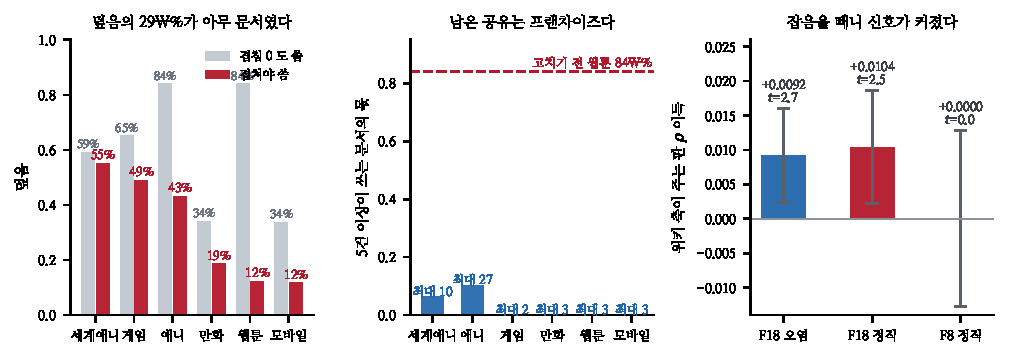
\includegraphics[width=\textwidth]{figs/match.pdf}
\caption{왼쪽 --- 덮음의 29\%가 아무 문서였다. 가운데 --- 남은 공유는
프랜차이즈다. 오른쪽 --- 잡음을 빼니 신호가 커졌다.}
\end{figure*}

\section{스물다섯 건을 눈으로 봤다}

한국어판을 붙이고 웹툰 스물다섯 건을 시험 삼아 긁었다. 채움이 21/25로
좋아 보였다. 그런데 붙은 문서를 찍어 보니 ---

\begin{table}[t]
\centering\tsize
\caption{고치기 전. 웹툰 표본 25건.}
\begin{tabular}{lrl}
\toprule
붙은 문서 & 건 & \\
\midrule
\textbf{네이버 웹툰} & \textbf{21} & 플랫폼 문서 \\
참교육 & 1 & 맞음(창은 빔) \\
못 찾음 & 3 & \\
\bottomrule
\end{tabular}
\end{table}

\claimx{\textbf{채움률만 봤으면 못 봤다.} 21/25는 세계애니(22/25)와 거의
같은 수치다. 값을 찍어 보고서야 스물한 건이 같은 문서라는 것이 보였다.}{노트
133 · 142에서 같은 자리에 두 번 걸렸다 --- 이름과 값이 갈리는 곳. 이번에는
``덮음''이라는 요약 하나가 스물한 건의 동일성을 감췄다.}

\section{29퍼센트였다}

\begin{table}[t]
\centering\tsize
\caption{겹침 0 으로 붙은 문서. 전체 감사.}
\begin{tabular}{lrl}
\toprule
& 건 & \\
\midrule
점수 1.0 (제목 같음) & 1{,}935 & \\
점수 0.8/0.9 (품음) & 552 & \\
\textbf{점수 0.0 (안 겹침)} & \textbf{1{,}002} & \textbf{29\%} \\
\bottomrule
\end{tabular}
\end{table}

\begin{table}[t]
\centering\tsize
\caption{겹침 0 이 간 곳.}
\begin{tabular}{llr}
\toprule
웹툰 & 네이버 웹툰 & 17 \\
모바일 & List of video games released in 2026 & 7 \\
모바일 & WhatsApp & 6 \\
만화 & List of yuri works & 5 \\
세계애니 & Tomoaki Maeno (성우) & 4 \\
모바일 & App store & 4 \\
\bottomrule
\end{tabular}
\end{table}

\claimx{\textbf{여러 레코드가 한 문서를 나눠 쓰면 그 축은 날짜만 잰다.}
같은 문서의 조회수를 서로 다른 창으로 자를 뿐이므로, 남는 변이는 시점뿐이다.
그것을 ``오픈 이전 관심도''라고 부르면 안 된다.}{그렇다고 공유가 다 나쁜
것은 아니다 --- 2기 · 3기가 프랜차이즈 문서를 같이 쓰는 것은 의도한 바다.
그래서 판정이 아니라 분포를 적는다.}

\section{한글이 지워지고 있었다}

\claimx{\textbf{정규화가 한글을 지웠다.} 비교용 정규화가
\texttt{[\^{}a-z0-9]} 를 전부 없애서 ``나 혼자만 레벨업''이 빈 문자열이
됐다. 빈 문자열은 아무것과도 안 겹치니 점수가 언제나 0이고, 그러면 위 규칙에
따라 \emph{모든} 한국어 제목이 검색 1위로 갔을 것이다.}{영문 도메인에서는
이 버그가 안 보인다. 한국어판을 붙이는 그 순간에만 터진다 --- 그리고 그때
100\%가 오염된다.}

\section{넷을 고쳤다}

\begin{table}[t]
\centering\tsize
\caption{고침.}
\begin{tabular}{ll}
\toprule
① & 겹침 0 이면 안 붙인다 (문서 없음으로 적는다) \\
② & 정규화가 한글을 남긴다 \\
③ & 오염된 1{,}002건을 지우고 다시 긁는다 \\
\textbf{④} & \textbf{\texttt{shared()} --- 한 문서를 몇이 쓰나를 상시로} \\
\bottomrule
\end{tabular}
\end{table}

\begin{table}[t]
\centering\tsize
\caption{고친 뒤. 나눠 쓰기.}
\begin{tabular}{lrrl}
\toprule
& 최대 & 5$+$ 몫 & 최대 공유 문서 \\
\midrule
애니 & 27 & 10.3\% & 원피스 (애니메이션) \\
세계애니 & 10 & 6.3\% & My Hero Academia \\
만화 & 3 & 0\% & \\
웹툰 & 3 & 0\% & \\
게임 & 2 & 0\% & \\
\bottomrule
\end{tabular}
\end{table}

\claimx{\textbf{남은 공유는 전부 프랜차이즈다.} 원피스 27건 · 명탐정 코난
16건 · 나의 히어로 아카데미아 13건 --- 장수 시리즈가 시즌마다 레코드를
갖고 문서를 하나 쓴다.}{웹툰의 ``연애''가 3건인데 이건 제목이 일반 명사라
한국어 위키의 다른 문서에 정확히 걸린 경우다. 제목 겹침만으로는 이런 것을
못 거른다.}

\section{씻으니 이득이 커졌다}

\begin{table}[t]
\centering\tsize
\caption{위키 축이 주는 판 $\rho$ 이득. 씨앗 셋 평균 · 짝 재추출 400.}
\begin{tabular}{lrrl}
\toprule
& 이득 & 짝 sd & \\
\midrule
F18 · 오염된 축 & $+$.0092 & .0034 & $t{=}2.7$ \\
\textbf{F18 · 씻은 축} & \textbf{$+$.0104} & \textbf{.0041} & \textbf{$t{=}2.5$} \\
F8 · 씻은 축 & $+$.0000 & .0064 & $t{=}0.0$ \\
\bottomrule
\end{tabular}
\end{table}

\claimx{\textbf{덮음은 29\% 줄었는데 신호는 늘었다.} $+$0.0092에서
$+$0.0104로. 지운 1,002건이 잡음이었다는 직접 증거다 --- 잡음 축은 이득을
깎는다.}{짝 sd 가 0.0034에서 0.0041로 늘어 $t$ 는 2.7에서 2.5로 조금
내렸다. 관측 수가 줄었으니 당연하다. 여전히 갈린다.}

\begin{table}[t]
\centering\tsize
\caption{도메인별. F18 배깅, 씻은 축.}
\begin{tabular}{lrrr}
\toprule
& 위키 덮음 & 현행 & $+$위키 \\
\midrule
\textbf{게임} & 49\% & $+$.410 & \textbf{$+$.472} \\
\textbf{세계애니} & 55\% & $+$.494 & \textbf{$+$.555} \\
애니 & 43\% & $+$.475 & $+$.483 \\
모바일 & 12\% & $+$.566 & $+$.562 \\
웹툰 & 12\% & $+$.358 & $+$.343 \\
팝업 & 0\% & $+$.451 & $+$.470 \\
\bottomrule
\end{tabular}
\end{table}

\claimx{\textbf{덮음이 얇으면 값진다.} 게임(49\%)과 세계애니(55\%)가
$+$0.06씩 오르고, 웹툰(12\%)과 모바일(12\%)은 조금 내린다. 축을 절반도 못
채우면 그 열은 관측된 소수에만 쓰이고 나머지는 중립으로 채워진다.}{팝업의
$+$0.019는 여전히 주장 안 한다 --- 팝업에는 위키 축이 없다(노트 144의
귀착 전파).}

\begin{table}[t]
\centering\tsize
\caption{남은 것.}
\begin{tabular}{ll}
\toprule
웹툰·모바일 & 덮음 12\% --- 붙일지 말지를 도메인마다 \\
일반 명사 & ``연애'' 같은 제목은 제목 겹침으로 못 거른다 \\
누수 & 웹툰 $|r|{=}.376$ 이 제일 높다 --- 문턱 아래지만 \\
\bottomrule
\end{tabular}
\end{table}

셋째 줄을 적어 둔다. 웹툰의 \texttt{wiki\_peak\_ratio} 와 라벨의 상관이
0.376으로 이 축 세트에서 제일 높다. 문턱 0.70 아래지만, 웹툰 라벨이 네이버
즐겨찾기이고 위키 조회수도 ``화제가 된 정도''를 재므로 같은 것을 두 번 재는
쪽에 가깝다. \textbf{덮음 12\%로 이득도 안 나니 웹툰은 안 붙이는 쪽이 낫다}
--- 다만 그 결정을 점수로 하면 노트 126이 잡은 그 잘못이니, 덮음 문턱으로
정하는 편이 맞다.

\end{document}
